%%%%%%%%%%%%%%%%%%%%%%%%%%%%%%%%%%%%%%%%%%%%
\subsubsection{Study Focal Plane using MCS [Daytime]}\label{secflow:prestudy}
In this process, we study the distortion of the focal plane using MCS, and check validity the PFS coordinate-transfer system.
This process is planned to use time efficiently after the PFI arrival, because, according to the current schedule (as of January 2017), MCS will be delivered to the Subaru telescope a year earlier PFI.

In this process , we will:
\begin{enumerate}
\item Align MCS on MCBox with respect to the Prime Focus (POpt2). [ASIAA work]
\item Verify image quality. [ASIAA work]
\item Study dome seeing effect. [ASIAA work]
\item Demonstrate MCS-F3C coordinate transformation, and
\item Study WFC distortion map in detail
\end{enumerate}
Note that the first three items is proposed by ASIAA in MCS CDR document : ({\tt MCS\_I\&T.pdf, and PFS MCS Delta CDR.pdf}),

Regarding the image quality, the similar test will be done in the process \ref{secflow:MCSperf}, where science and fiducial fibers are used.
Hence, if the image quality will be validated well enough in this process, we may skip \ref{secflow:MCSperf}.
but note that it is still worth validating the image quality with real fibers.

Since PFI will not available for this process, we have two options as an alternative.
One is Echidna positioner system of FMOS/PIR, and the other is pinhole array equipped to POpt2.
Table \ref{tbl:fmos_pinhole} summarizes the specifications of Echidna on FMOS/PIR and pinhole on POpt2 as well as their usefulness for tests in this sequence. 
{\bf At discussion on AIT work in October 2016, it was decided that we will use pinhole array on POpt2. }

\paragraph{In the case of FMOS/PIR}
The field of view of FMOS/PIR ($\sim$ 150mm $\times$ $\sim$ 150mm, corresponding to $\sim 30$ arcmin in diameter) is much smaller than that of PFS, and their optics and mechanics are different from each other.
Besides, only 32 fibers out of 400 can be back-illuminated simultaneously.
These facts imply that Echidna on FMOS/PIR is not suitable for the MCS alignment and image quality test.
Nonetheless, the procedure of coordinate transformation shall be studied well.

MCS measures fiber positions somewhat converted to MCS frame, and then positions are transferred to them on focal plane.
On the other hand, FMOS fiber positioner (Echidna) measures fiber positions on the focal plane.
By comparing measured fiber positions by MCS and the coordinate transformation system, with those by Echidna, MCS function of measuring the fiber positions is verified.
%The error in measurement contributed by dome seeing temperature, or telescope elevation will be also estimated by measuring position several elevation and temperatures.
%% estimation of error is needed for PFI-MCS relation? maybe not. but error estimation is needed for measurement on MCS?
%% Echidna: 20 fibers are illuminated at a time
At present, Echidna can position fibers with the accuracy of $\sim 35$ um\footnote{Originally the fiber allocation was achieved with the accuracy of $\sim 10$um. Recently the encoder of X position of sky camera was broken, which have added $\sim 25$ um for fiber positions.}.
We set the goal in accuracy of fiber positioning 50 um for pre-study, the same as 1-st pass distortion map (\ref{secflow:1stDM}).

The procedure of the measurement is as follows:
\begin{enumerate}
\item Decide which fibers to move and which fibers not to move (like fixed fiducial fibers).
Figure \ref{fig:fibEchidna} shows an example.
%One way is to define  nine fixed fibers arranging 3 $\times$ 3 grid. 
\item Built distortion map of PIR from the MCS viewpoint (the form of $D_2$ for FMOS/PIR).
With all fibers back-illuminated, we take the fiber image at home position by MCS.
We also have the physical positions of FMOS fibers.
Using these positions, we will determine the form of the distortion map.
\item Define F3C for FMOS. 
In order to distinguish with F3C for PFS, we name the defined coordinate ``F3C(PIR)". 
``F3C(PIR)" is practically the same as the positions measured with the spine camera of Echidna.
With fixed fibers back-illuminated, we take fibers image by both MCS and Echidna, and then the positions of fixed fiducial fibers on F3C are measured.
\item Take all fibers image by MCS and calculate their position
\begin{enumerate}
\item Using image of fixed fibers, determine the transformation from MCS coordinate to F3C(PIR) coordinates, that is, the parameters of $D_2$ for FMOS/PIR). 
\item Using images of the rest fibers, calculate the positions on above coordinate frame.
\end{enumerate}
\item Measure fiber positions of FMOS/PIR, and compare with those derived on F3C(PIR)
\item Executing the above procedures for several fiber configurations at a various Elevation (EL) and Rotator angle (ROA), study the stability of the measurements.
We may be able to study the effect of local surface error of corrector lens for coordinate transform by changing fiber configurations.
Here the error due to temperature and dome seeing is included.
We also examine these effect.
\end{enumerate}

%--------------------------------------------------------------
%  Figure: An example of fiber arrangement 
%--------------------------------------------------------------
\begin{figure}[!ht]
\begin{center}
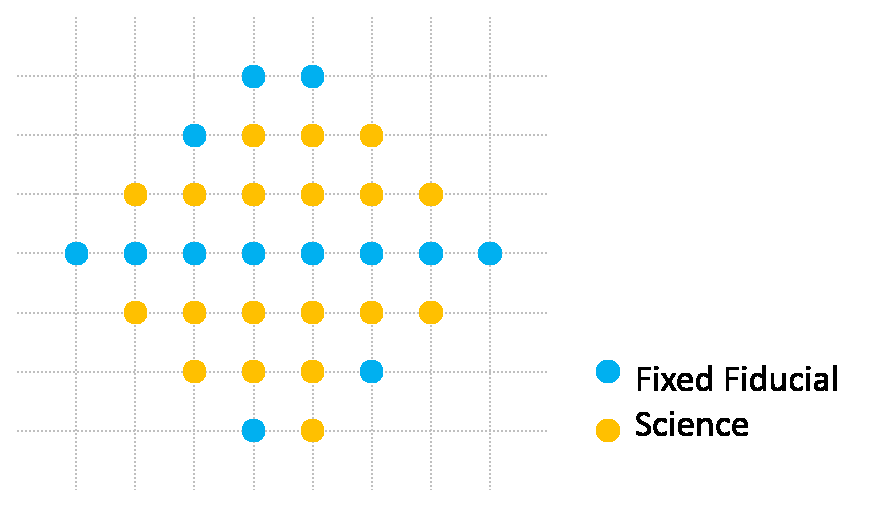
\includegraphics[width=90mm]{fiber_echidna.eps}
\end{center}
\caption{
Example of the arrangement of FMOS/Echidna back-lit fibers.
32 fibers can be back-illuminated at a time. }
\label{fig:fibEchidna}
\end{figure}

Because the corrector lens are different between PIR and WFC, we cannot study a effect of WFC surface figure error itself if we use FMOS.
However, similar study will be performed by changing the fiber configurations (TBC).

\paragraph{In the case of pinhole array on POpt2}
If pinhole array can be attached on the POpt2, we can of course align MCS and test image quality.
Also we can study transfer coordinate system in the similar procedure above.
WFC has a ring-patterned local surface error with a pitch of 6mm, we can study the effect of the local surface error on WFC distortion by using pinholes with the smaller pitch, or rotating pinholes slightly.

Supposing that we will have pinhole mask with holes arranged at fiducial fiber position and hexagonal position of 4 mm (half of the pitch of  Cobras), we will study the coordinate transform in the following procedure.
\begin{enumerate}
\item Distortion map is determined with WFC as-built model.
\item \label{item:M4pin2} Take pin holes array images by MCS.
Choose one of the holes in the patrol areas and calculate their position on F3C.
\item Compare the calculated positions with the design.
\item Choosing the another holes, repeat \ref{item:M4pin2}.
\item Executing the above procedures at a various Elevation (EL) and Rotator angle (ROA), study the stability of the measurements.
Since the existing as-build models are at only three elevations (EL=90$\degree$, 60$\degree$, and 30$\degree$), we will modify the distortion map using the data at other elevations.
\end{enumerate}

Although the pinhole array prepared by ASIAA has the 8mm pitch (partly 2mm), we can use the ASIAA pinhole for the above by rotating the instrument slightly.
The movement accuracy of the instrument rotator of POpt2 is 8 arcsec, enough smaller than angle corresponds to 8 mm at the field edge (at 250 mm radius, $\sim$ 1.8$\degree$ ).
This pinhole size is $\sim$ 356mm $\times$ $\sim$ 356mm, which covers $\sim 75\%$ of FoV of WFC.
The diagonal length 497.84 mm is larger than the circumcircle of AG cameras (496 mm in diameter).
Therefore, distortion shall be studied well.

To minimize (and measure) the effect of dome seeing, we will take 100 frames for a given position.
Assuming that it takes $\sim$10 seconds, it will take about 20 minutes to obtain the data at a given position.
For study of distortion map, we will take data at 7 elevation angles (with 10$\degree$ step from EL=90$\degree$ to 30$\degree$).
To cover the entire FoV, we have to arrange the pinhole array at three azimuth angles.
It will, therefore, take 7 hours to obtain the data.
To study the effect of WFC surface figure error on the coordinate transformation, we will take 5 sets of 100 frames by moving the instrument rotator slightly.
If we will study this at 5 elevations (with 15$\degree$ step from EL=90$\degree$ to 30$\degree$), it will take about 8.3 hours.
In total, 2-day are required for this step.

%---------------------------------------------------
% Table: Comparison b/w FMOS/PIR and pinhole/POpt2
%---------------------------------------------------
\begin{table}[!ht]
\begin{center}
\caption{Specifications of Echidna on FMOS/PIR and pinhole on POpt2, and their usefulness.
%Note that we assume that pinhole mask is the same type as ASIAA.
}
\label{tbl:fmos_pinhole}
%\scriptsize
%\footnotesize
\begin{tabular}{p{35mm}|*{3}{|p{40mm}}} \hline
Specifications	& Echidna on FMOS/PIR & Pinhole on POpt2 & Requiring Test Items\\ \hline \hline
Size at focal plane	& $\sim$150mm $\times$ $\sim$150mm (at field center)		& $\sim$356mm $\times$ $\sim$356mm ($\sim 75 \%$ PFI FoV)	& distortion \\ \hline
Optics and mechanics	& FMOS specific	& WFC + POpt2 itself	& alignment, image quality, distortion, MCS-PFI coordinate transformation \\  \hline
Expected focal-plane spatial sampling rate	& $\sim$ 35 um	& $\sim$ 10um (at field edge)	& distortion \\ \hline
RMS spot radius on MCS detector(*)	& $\sim$10 um at field center, $\sim$20um at field edge	& $\sim$ 9um	& image quality \\ \hline
\end{tabular} 
\end{center}
* : MCS CDR document ({\tt PFS MCS Delta CDR.pdf} by S.-Y. Wang.)
\end{table}

\paragraph{Back-up plan}
If MCS would deliver at Subaru just before the arrival of PFI, we will not have enough time to practice the procedure of the coordinate transformation.
As back-up plan, we will use the camera which was used to measure dome seeing in 2012.

According to the report (http://sumire.pbworks.com/w/file/70195197/domeseeing3v1.pdf), the camera was equipped to the Caseggrain focus with NexStar4SE telescope.
In this configuration, the camera covers 100 mm $\times$ 120 mm of FMOS focal plane, which is large enough to illuminate 32 fibers, because neighboring fibers have 7mm separation.
The FWHM of the spot size on the camera will be 2.6 pixel, which is the same as that of the PFS fibers on MCS.

\paragraph{Designated Tool for This Process}
For function of MCS-PFI coordinate transformation, we will use the first version for the scientific operation.
For measurement of spot measurement, we will use MCS software itself.
To check coordinate transformation algorithm, we will prepare a software to choose the fiducial spots and science spots.

\begin{itembox}[l]{\suctitle{Success Criteria}}
MCS measures the fiber position consistent with pinhole array spacing at various telescope positions. 
The accuracy is less than 50 um.

\bluetext{Required long time to analyze the data?: Yes. \\
---It should take time to compare the positions derived with MCS with pinhole array, and mature the coordinate transfer algorithm.
Once we obtained the data, we can use the same data to mature the algorithm.
}
\end{itembox}